\documentclass[]{beamer} 
\setbeamerfont{all}{size=\large}
\setbeamerfont*{itemize/enumerate body}{size=\large}
\setbeamerfont*{itemize/enumerate subbody}{parent=itemize/enumerate body}
\setbeamerfont*{itemize/enumerate subsubbody}{parent=itemize/enumerate body}
\beamertemplatenavigationsymbolsempty
\usetheme{default}
\useinnertheme{circles}
\usebeamerfont{all}
\DeclareMathOperator*{\argmin}{arg\,min}
\usepackage{listings}
\usepackage{amssymb}
\usepackage{amsmath}
\usepackage{docmute}
\usepackage{hyperref}
\begin{document}

%\hspace*{\fill} \\

\title{In-network Upsampling with Convolutional Nets}
\author{Nicholas Dronen}


\begin{frame}
\maketitle
\end{frame}


\begin{frame}{Transposition and Networks}
Error is propagated back through e.g. a multi-layer perceptron via transposition of weight matrices. \\
\vspace{2mm}
\centering
On the forward pass for a layer $\ell$,
\begin{equation*}
z^{\ell} = \sigma(x\mathbf{M}_{\ell} + b_{\ell}).
\end{equation*}
Then, going backward, 
\centering
\begin{equation*}
\delta^{\ell} = \mathbf{M}^{\color{red}{T}} \delta^{\ell+1} \odot {z^{\ell}}^{\prime}.
\end{equation*}
\end{frame}


\begin{frame}{Transposition with 1d Convolutions}
Let $x \in R^{k \times 1}$ and $\mathbf{H} \in R^{d \times k}$ be a Toepliz matrix representation of a filter $h \in R^{k}$. \\
\vspace{2mm}
\centering
On the forward pass,
\begin{equation*}
y = \mathbf{H} x.
\end{equation*}
And going backward (assume $\mathbf{H}$ is orthogonal),
\begin{equation*}
x = \mathbf{H}^{\color{red}{T}} y.
\end{equation*}
\end{frame}


\begin{frame}{Discrete Convolution - 2d}
\centering
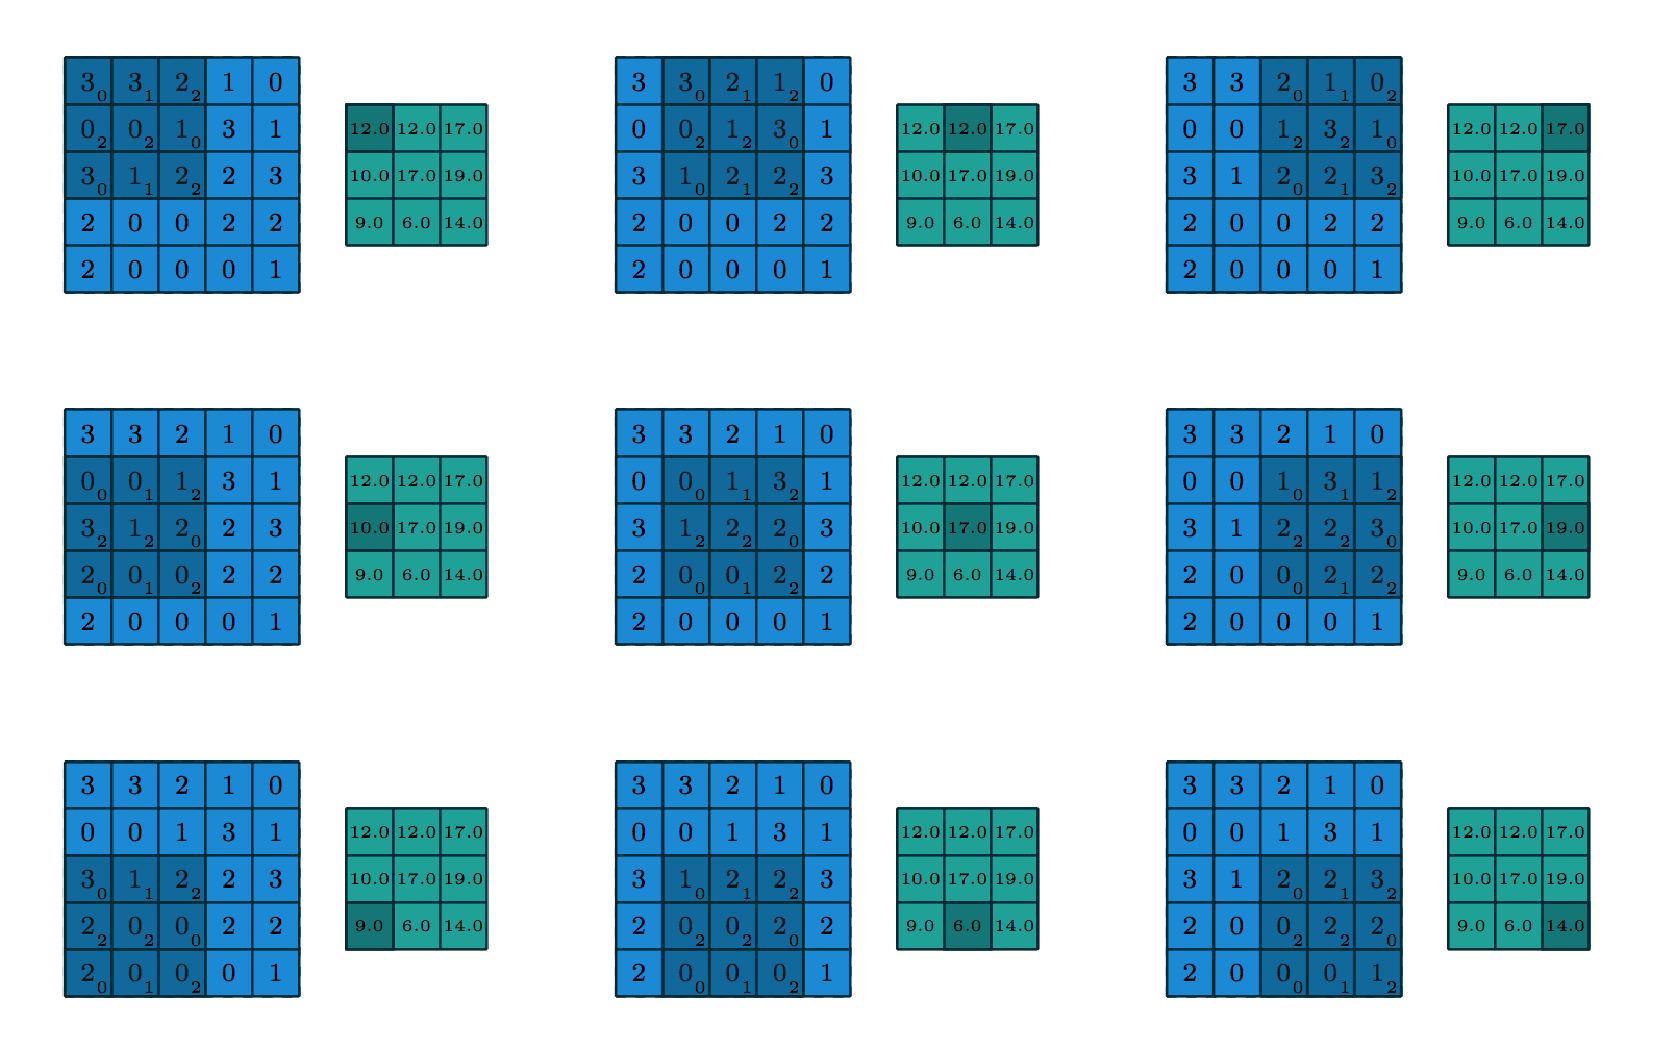
\includegraphics[scale=0.325]{figures/discrete-convolution} \\
\href{https://arxiv.org/abs/1511.07122}
{\textcolor{blue}{A guide to convolution arithmetic for deep learning, Dumoulin and Visin, arXiv:1603.07285 [stat.ML]}}
\end{frame}


\begin{frame}{Transposed Convolution - 2d}
\centering
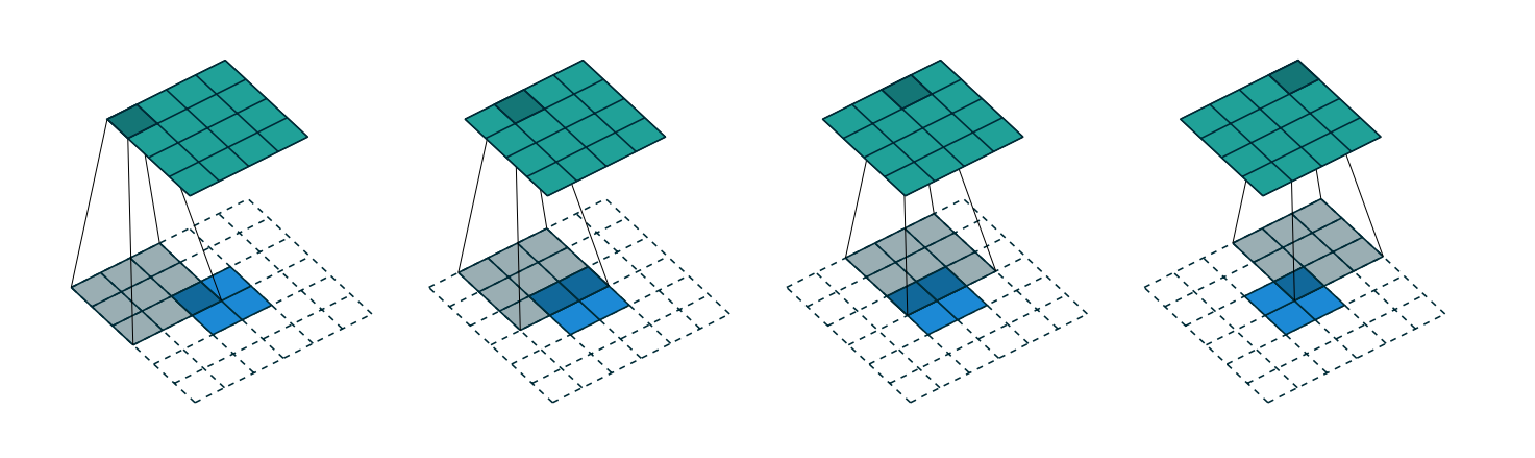
\includegraphics[scale=0.325]{figures/transposed-convolution} \\
\href{https://arxiv.org/abs/1511.07122}
{\textcolor{blue}{A guide to convolution arithmetic for deep learning, Dumoulin and Visin, arXiv:1603.07285 [stat.ML]}}
\end{frame}


\begin{frame}{Transposed Convolution}
\centering
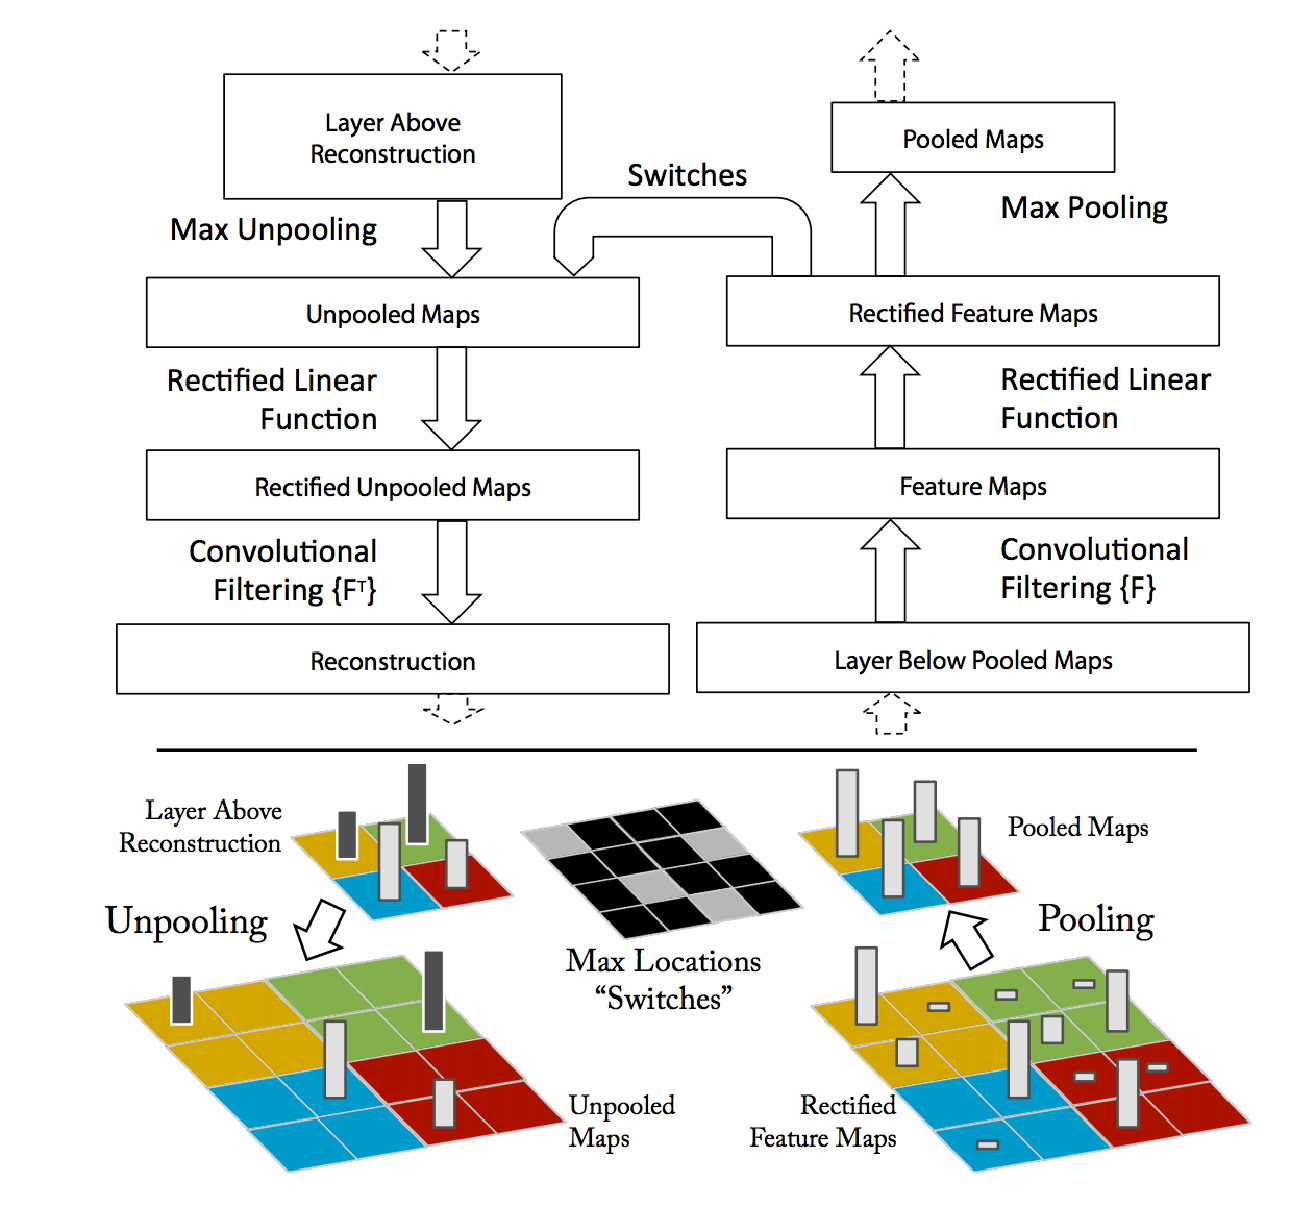
\includegraphics[width=0.75\textwidth]{figures/zeiler-transposed} \\
\href{https://arxiv.org/abs/1311.2901}
{\textcolor{blue}{Visualizing and Understanding Convolutional Networks, Zeiler and Fergus, arXiv:1311.2901 [cs.CV]}}
\end{frame}


\begin{frame}{Subpixel Convolution}
\centering
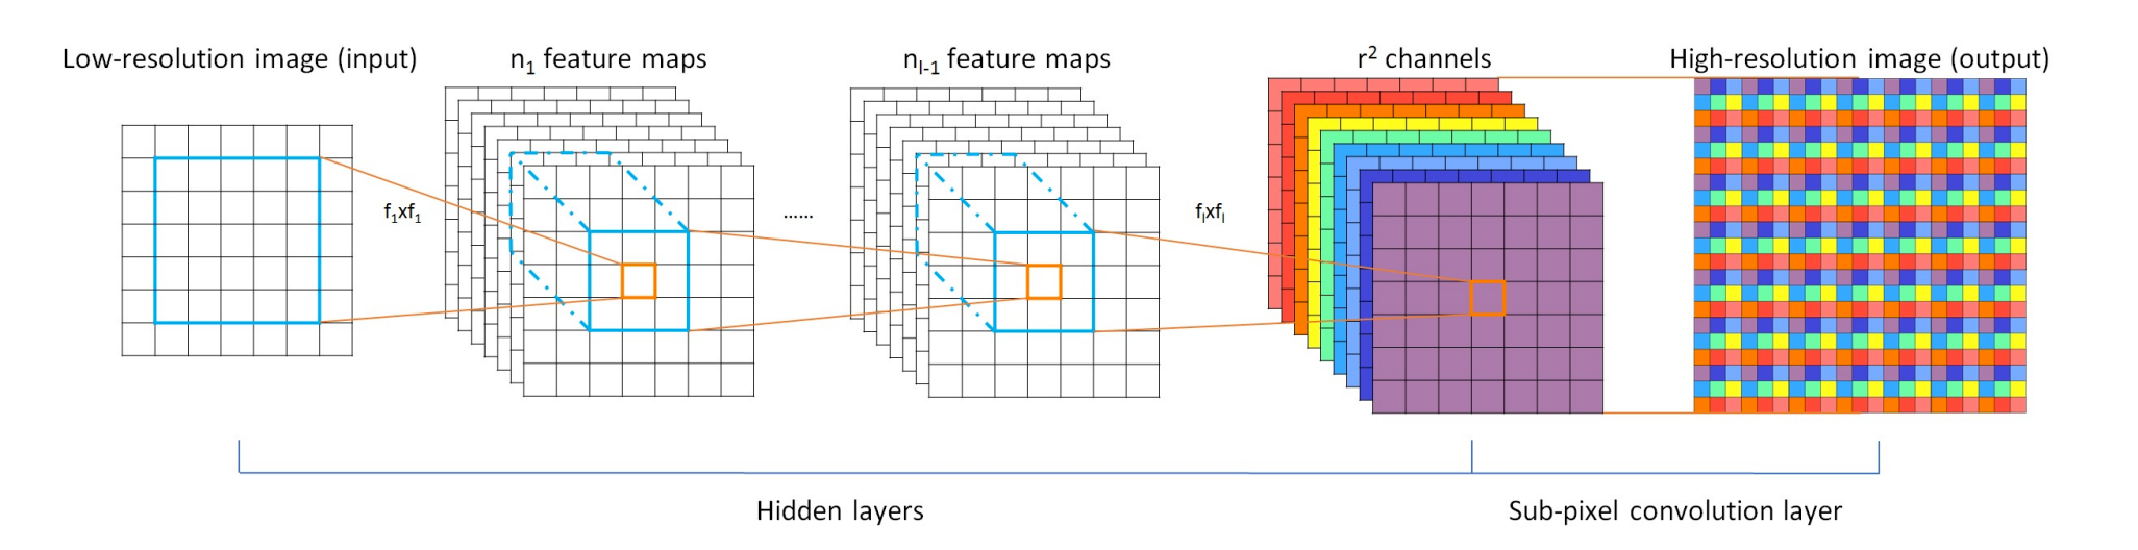
\includegraphics[width=0.85\textwidth]{figures/shi-subpixel} \\
\href{https://arxiv.org/abs/1609.05158}
{\textcolor{blue}{Real-Time Single Image and Video Super-Resolution Using an Efficient Sub-Pixel Convolutional Neural Network, Shi et al, arXiv:1609.05158 [cs.CV]}}
\end{frame}


\begin{frame}{Subpixel Convolution}
\centering
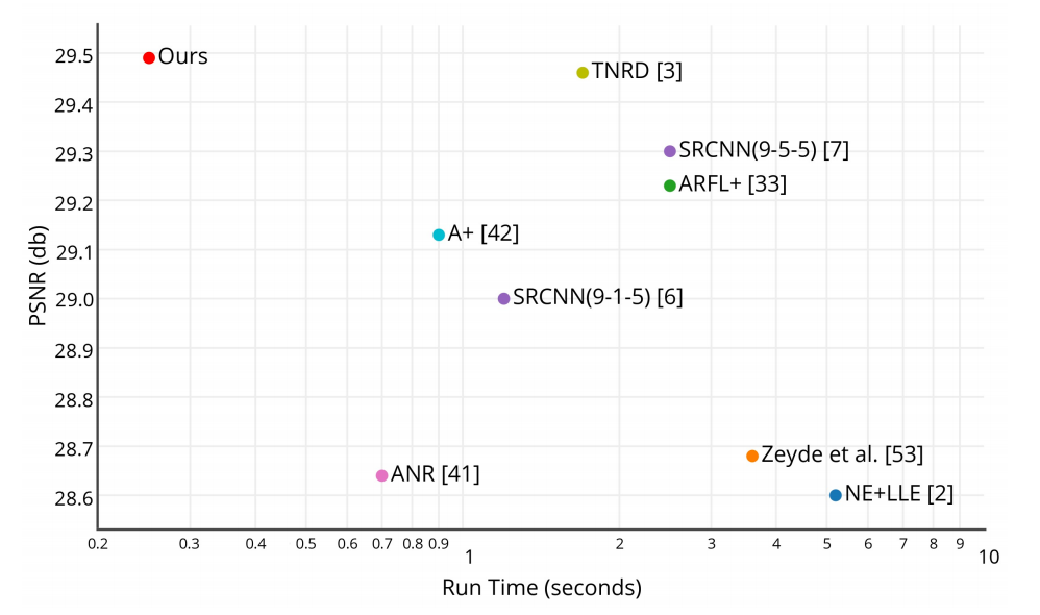
\includegraphics[width=0.85\textwidth]{figures/shi-subpixel-trade-off} \\
\href{https://arxiv.org/abs/1609.05158}
{\textcolor{blue}{Real-Time Single Image and Video Super-Resolution Using an Efficient Sub-Pixel Convolutional Neural Network, Shi et al, arXiv:1609.05158 [cs.CV]}}
\end{frame}


\begin{frame}{Transposed vs. Subpixel Convolutions}
\centering
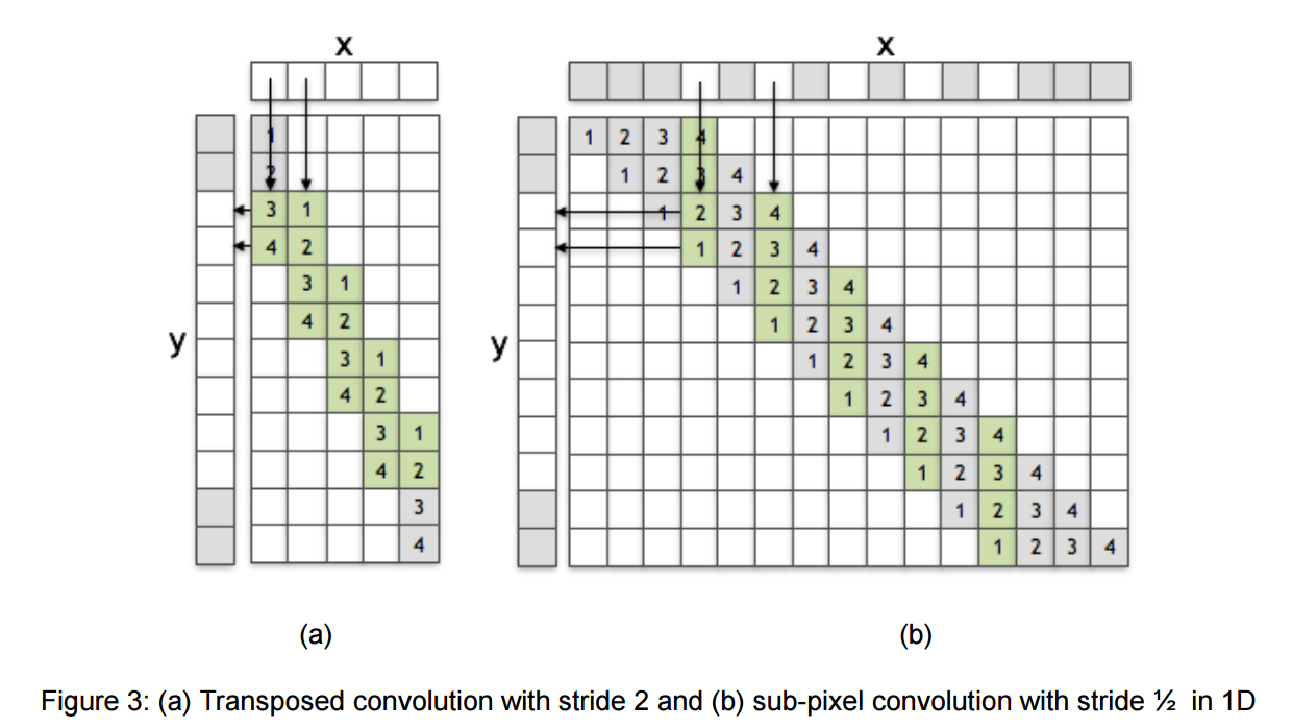
\includegraphics[width=0.85\textwidth]{figures/shi-subpixel-vs-transposed} \\
\href{https://arxiv.org/abs/1609.07009}
{\textcolor{blue}{Is the deconvolution layer the same as a convolutional layer?, Shi et al, arXiv:1609.07009 [cs.CV]}}
\end{frame}


\begin{frame}
\begin{itemize}
\item Experimental setup (task, data, framework, models)
\item Quantitative results (use PSNR (db) not MSE)
\item Qualitative results
\item Error analysis
\item Performance analysis
\item Availability of code (source file and Jupyter notebook)
\item Visualizations of filter weights and biases?
\end{itemize}
\end{frame}

\end{document}
